% !TeX spellcheck = de_DE
%_______________________________________________________________________________
%class
%_______________________________________________________________________________
%\documentclass[a4paper,11pt,onecolumn,final,german,openbib]{scrbook}
\documentclass[a4paper,11pt,oneside,final,german,openbib,pdftex]{scrbook}
%_______________________________________________________________________________
% page borders
%_______________________________________________________________________________
\addtolength{\headheight}{2cm}
%\addtolength{\topmargin}{2cm}
\setlength{\oddsidemargin}{1.0cm}
\setlength{\evensidemargin}{0.5cm}
\setlength{\textwidth}{14.3cm}
\setlength{\parindent}{0mm}

%_______________________________________________________________________________
% packages
%_______________________________________________________________________________
\usepackage{german}
\usepackage{amsmath, amssymb}
\usepackage[utf8]{inputenc}
\usepackage{graphicx}
\usepackage{enumerate}
\usepackage{multirow}
\usepackage{subfigure}
\usepackage{dsfont}
\usepackage{slashed}
\usepackage{textcomp}
\usepackage{url}
\usepackage{hyperref}
\usepackage{endnotes}




%_______________________________________________________________________________
% bold fonts for headings
%_______________________________________________________________________________
\font\afont=cmssbx10 scaled \magstep5     % for the title
\font\bfont=cmssbx10 scaled \magstep4     % for chapter headings
\font\cfont=cmssbx10 scaled \magstep3
\font\dfont=cmssbx10 scaled \magstep2     % for section headings and author name
\font\efont=cmssbx10 scaled \magstephalf

%_______________________________________________________________________________
% index depth
%_______________________________________________________________________________
\setcounter{secnumdepth}{3}
\setcounter{tocdepth}{3}

%_______________________________________________________________________________
% new commands
%_______________________________________________________________________________
\newcommand{\demi}{\frac{1}{2}}

%_______________________________________________________________________________
% renewed commands
%_______________________________________________________________________________
% \renewcommand{\topfraction}{1.}       % this is important for figure placement
% \renewcommand{\bottomfraction}{1.}
\makeatletter
\renewcommand\paragraph{\@startsection{paragraph}{4}{\z@}%
  {-3.25ex\@plus -1ex \@minus -.2ex}%
  {1.5ex \@plus .2ex}%
  {\normalfont\normalsize\bfseries}
}
\makeatother

%_______________________________________________________________________________
% special words, hyphenation
%_______________________________________________________________________________
\hyphenation{Ba-che-lor-ar-beit}

\pagestyle{empty}
\pagestyle{headings}
%for changing the style on a specific page use \thispagestyle{e.g., empty}

%_______________________________________________________________________________
%_______________________________________________________________________________
\begin{document}
\pagenumbering{roman}

%_______________________________________________________________________________
\begin{titlepage}
  \vspace*{6mm}
  \begin{center}
     {\afont Systematische Studien zur $\pi^0$ Kalibrierung des Crystal-Ball Detektor}
     \\[3.5cm]
     {\large von}
     \\[3.5cm]
     {\dfont Martin Sobotzik}
     \\[2cm]
     {\large Bachelorarbeit in Physik \ rtm/\\
        vorgelegt dem Fachbereich Physik, Mathematik und Informatik (FB 08) \/\\
        der Johannes Gutenberg-Universit\"at Mainz \/\\
        am 1. April 2012}
   \end{center}
   \vfill
   1. Gutachter: Prof. Dr. Wolfgang Gradl\\	
   2. Gutachter: Prof. Dr. Achim Denig \\
   \vfill
\end{titlepage}

\thispagestyle{empty}
Ich versichere, dass ich die Arbeit selbstst\"andig verfasst und keine 
anderen als die angegebenen Quellen und Hilfsmittel benutzt sowie 
Zitate kenntlich gemacht habe.
\\
\\[3.5cm] 
Mainz, den [Datum] [Unterschrift]
\vfill
\noindent 
Martin Sobotzik\\
KOMET\\
Institut f\"ur Physik\\
Staudingerweg 7\\
Johannes Gutenberg-Universit\"at
D-55099 Mainz\\
{\url{ msobotzi@students.uni-mainz.de}}

%_______________________________________________________________________________
\renewcommand\contentsname{Inhaltsverzeichnis}
\renewcommand\figurename{Abbildung}
\renewcommand\tablename{Tabelle}
\tableofcontents
\clearpage

\mainmatter
\sloppy

%_______________________________________________________________________________
\chapter{Einleitung}

\section{Motivaton}
{
	Diese Bachelorarbeit beschäftigt sich mit Studien zur Kalibrierung des Crystal-Ball Detektors der A2-Kollaboration am Institut für Kernphysik an der Johannes-Gutenberg-Universität.
	Die A2-Kollaboration untersuchte unter anderem die innere Struktur von Nukleonen mit Hilfe eines, durch Bremsstrahlung erzeugten, reellen Photonenstrahls. 
	
	Wird ein hochenergetisches Photon durch ein Proton absorbiert, werden Stark-Wechselwirkende Teilchen erzeugt. Diese Teilchen zerfallen überwiegend in Photonen, welche schließlich mit dem Crystal-Ball Detektor nachgewiesen werden können. 
	
	Der Crystal-Ball bestand aus 672 Natriumiodid Kristallen die als Detektoren dienten und deckte ca. 94\% des Raumwinkels ab.
	Er hatte zwei Bereiche ohne Detektor die für den Strahlenein und -ausgang vorheriger Experimente dienten.
	Um die Detektoren nun zu kalibrieren, betrachtete man folgende Prozesse:
\begin{equation}
	\gamma + p \rightarrow p + \pi^0
	\label{eq.gammascattering}
\end{equation} 
Bei diesem Prozess absorbiert ein Proton $p$ ein hochenergetischen Photon $\gamma$. Dabei wird ein $\pi^0$-Meson erzeugt.

	\begin{equation}
		\pi^0\rightarrow \gamma \gamma
		\label{eq.pi0decay}
	\end{equation}
	Das $\pi^0$-Meson zerfällt direkt zu 98,8\% in zwei Photonen und zu ca. 1,2\% in $e^+e^-+\gamma$. Andere Modi können vernachlässigt werden, da sie nur Wahrscheinlichkeiten von unter $10^{-5}$\% aufweisen. Im Crystal-Ball wurde, sowohl die Energie der Photonen, als auch ihr Winkel in Strahlrichtung bestimmt, woraus sich die invariante Masse des $\pi^0$ berechnen lies. 
	
	Eine Problematik ergab sich allerdings dadurch, dass zum Beispiel, ein Photon nicht seine gesamte Energie an einen Detektorkristall überträgt, sondern auch an die umliegenden. Nun hat aber nicht jeder Detektor gleich viele Nachbarn. Die Detektoren am Rand des Strahlenein- und ausgangs haben weniger Nachbarn, als die restlichen Detektoren. Folglich konnten sie nicht sehr gut kalibriert werden, da die Energie des Photons, welches diese Detektoren traf nicht vollständig bekannt war.
	
	Die Masse des $\pi^0$ ist mit 135 MeV wohl bekannt, folglich wurden die Detektoren so eingestellt, dass sich der $\pi^0$-Peak bei dieser Energie befindet. 
	\newline	 
	
	
%In der Einleitung Ihrer Bachelorarbeit sollte das Thema der Arbeit 
%m\"oglichst allgemeinverst\"andlich eingef\"uhrt werden. Gehen Sie 
%dabei auch auf das weitere Umfeld der Arbeit ein und erl\"autern Sie, 
%warum Aufgabenstellung und Herangehensweise interessant sind. Auch 
%die weitere Gliederung kann angesprochen werden, um dem Leser einen 
%ersten \"Uberblick \"uber den nachfolgenden Text zu geben.
\section{Gliederung}

Die Gliederung
%_______________________________________________________________________________


\chapter{Das $\pi^0$ Meson}



\chapter{Experimenteller Aufbau am MAMI}




%_______________________________________________________________________________

Der Mainzer Mikrotron (MAMI) war zur Zeit meiner Bachelorarbeit ein mehrstufiger Rennbahn-Teilchenbeschleuniger (RTM\footnote{Race-Track-Microtron}) für Elektronenstrahlen und stand verschiedenen Arbeitsgruppen
 für Experimente zur Verfügung. Die Anlage befand sich auf dem Gelände des Instituts für Kernphysik (KPh) der Johannes Gutenberg-Universität 
und bestand aus mehreren Hallen.

Die A2-Kollaboration untersuchte vor allem die Struktur von Nukleonen mit Hilfe von reellen Photonen, welche durch Bremsstrahlung des MAMI-Elektronenstrahls erzeugt wurden. Die Photonenenergie konnte durch eine Photonenmarkierungsanlage (Tagger\footnote{to tag = markieren}) bestimmt werden. Nach der Reaktion mit dem Target wurden die Teilchen durch ein System von verschiedenen Teilchendetektoren nachgewiesen.

\begin{figure}[h]
	
	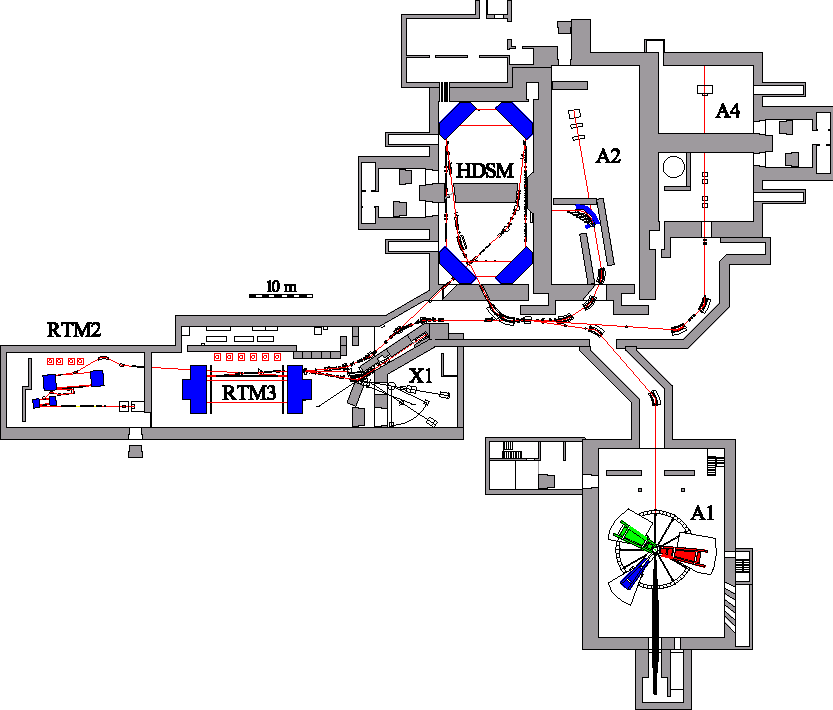
\includegraphics{grundriss}
	\caption{Grundriss der Beschleunigeranlage MAMI. Zu sehen sind die drei RTMs, der HDSM der Tagger und die verschiedenen Experimentierhallen: A1 (Elektronenstreuung), A2 (Strukturanalyse von Nukleonen), A4 (Parit\"atsverletzung) und X1 (R\"ontgenstrahlung). \cite{KPh07}}
	\label{fig.grundriss_anlage}
\end{figure}


\section{Der MAMI-Beschleuniger}
1979 wurde das MAMI erstmals in Betrieb genommen und bestand damals nur aus einem einzelnen RTM, womit eine maximale Elektronenenergie von 14 MeV erreicht werden konnte. 
Im Laufe der Jahre wurde das MAMI um zwei weitere RTMs und einem HDSM\footnote{Harmonic Double Sided Microtron} erweitert, wodurch eine Elektronenenergie von 1,5 GeV erreicht werden konnte.\cite{KPh11G} 
\newline


Um unpolarisierte Elektronen zu erzeugen, wurde eine Glühkathode auf 1000°C erhitzt. Dadurch konnten Elektronen den Heizdraht, aufgrund ihrer thermischen Bewegung, verlassen. Diese Elektronen wurden dann durch ein elektrisches Feld, welches durch die heiße Kathode und einer Anode, erzeugt wurde, zur Anode beschleunigt und traten dann durch ein Loch in der Anode aus und wurden weiter durch einen Linearbeschleuniger mit einer Frequenz von 2,45 GHz auf ca. 3,5 MeV beschleunigt. Diese Frequenz ist für das MAMI typisch und machte es zu einem Dauerstrich-Elektronen-Beschleuniger. Das heißt die Frequenz, mit der die Elektronen-Pakete auftraten, war größer, als die Frequenz, mit der die Detektoren einzelne Events auflösen konnten und somit wirkte der Strahl für die Detektoren kontinuierlich.
Am MAMI war es auch m\"oglich einen spinpolarisierten Elektronenstrahl zu erzeugen, dazu wurde ein GaAs Kristall mit polarisiertem Laserlicht bestrahlt.
\newline
Da die Elektronen mit einem Linearbeschleuniger nur einige MeV pro Meter beschleunigt werden k\"onnen, und man keine kilometerlangen Strecke bauen wollte, entschied man sich daf\"ur, die Elektronen mehrmals durch den gleichen Beschleunigerabschnitt zu beschleunigen. Dazu wurden sie nachdem sie beschleunigt wurden, durch zwei 180° Dipole so umgeleitet, dass sie wieder am Anfang des Beschleunigerabschnitts waren und diese Bahn abermals durchlaufen konnten. Nun besa{\ss}en die Elektronen mehr Energie und wurden in einer Bahn mit gr\"o{\ss}erem Radius durch die Dipole geleitet bis die gew\"unschte Energie erreicht wurde und der Strahl in den n\"achsten Abschnitt umgeleitet wurde. Die Struktur eines RTM erinnerte an eine antike Pferderennbahn, daher hat der RTM seinen Namen.

 Eine phasengerichtete R\"uckkopplung ist allerdings nur m\"oglich, wenn die statische und die dynamische Koh\"arenzbedingung erf\"ullt sind. Damit die statische Koh\"arenzbedingung erf\"ullt ist, muss die L\"ange der ersten vollst\"andigen Bahn ein ganzzahliges Vielaches der beschleunigten Hochfrequenz sein. F\"ur die dynamische Koh\"arenz muss die L\"angendifferenz von zwei aufeinander folgenden Uml\"aufen ebenfalls ein ganzzahliges Vielfaches der Wellenl\"ange sein\cite{Un08}. Diese Bedingungen gaben ebenfalls die Grenzen f\"ur den maximal m\"oglichen Energiegewinn jeder Stufe an. 
\newline
\newline
Wie bereits erw\"ahnt besa{\ss} MAMI drei dieser RTMs. Die erste Stufe MAMI A bestand aus zwei RTMs mit 18 bzw. 51 Uml\"aufen. Die zweite Stufe MAMI B bestand aus dem, zu diesem Zeitpunkt, gr\"o{\ss}ten RTM der Welt mit 90 Uml\"aufen und Dipolen mit einer Breite von jeweils 5 m, wodurch sie 450 t schwer waren. Damit waren auch die technischen Grenzen erreicht.\cite{KPh11F}


\begin{figure}[h]
	\begin{center}
	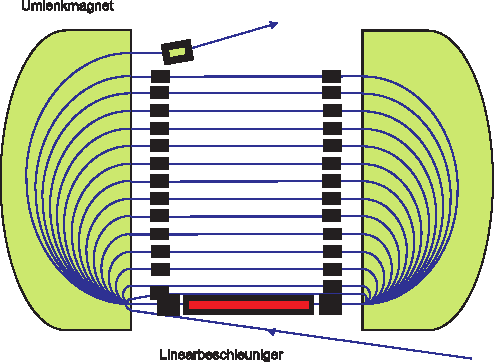
\includegraphics{RTM}	
	\caption{Prinzip eines RTM: Der Elektronenstrahl wird immer wieder durch den Linearbeschleuniger geschickt, bis die gew\"unschte Energie erreicht wurde und der Strahl mittels eines sogenannten Kicker-Magnet zum n\"achstem Abschnitt weiter geleitet wird.\cite{KPh07} }
	\label{fig.RTM}
\end{center}
\end{figure}

Um nun aber trotzdem h\"ohere Energien zu erreichen, musste sich ein neues Konzept \"ubelegt werden. MAMI C war folglich kein RTM mehr, sondern ein HDSM. Das hei{\ss}t, es bestand aus vier 90° Dipolen, welche jeweils 250 t schwer waren und einem zus\"atzlichen Linearbeschleuniger. F\" dieses HDSM wurde der erste Linearbeschleuniger der Welt gebaut, der mit einer Fequenz von 4,9 GHz betrieben werden konnte betrieben wurde er allerdings, wie die beiden voherigen RTMs mit einer Frequenz von 2,45 GHz.
\newline
\begin{table}[h]
	\begin{center}
		\begin{tabular}{|l|c|c|c|c|}
			\hline
			& RTM1 & RTM2 & RTM3 & HDSM \\
			\hline
			\hline
			Eingangsenergie &3,455 MeV  &  14,35 MeV& 179,5 MeV  &854,6 MeV \\ \hline
			Ausgangsenergie &14,35 MeV  &  179,5 MeV &854,6 MeV  & 1,5 GeV \\ \hline
			Anzahl Uml\"aufe&18  &51  &90  &43 \\ \hline
			Energiegewinn pro Umlauf &0,559 MeV  & 3,24 MeV & 7,5 MeV  & 13,93-16,63 MeV \\ \hline
			
	
		\end{tabular}
		\caption{Technische Daten der MAMI-Beschleunigerstufen \cite{Un08}}
		\label{tab.MAMIstufen}
	\end{center}
\end{table}


 Der Elektronenstrahl hatte am Ende der Beschleunigung eine Energie von ca. 1,5 GeV, diese konnte in etwa 15 MeV Schritten eingestellt werden. Sein Durchmesser lag im Mikrometerbereich, was sehr gute Voraussetzungen f\"ur Pr\"azisionsexperimente waren.\cite{KPh07}. 
 
 
 \section{Die Photonenmarkierungsanlage}
 
 In der A2-Experimentierhalle wurde der reelle Photonenstrahl mittels Bremsstrahlung erzeugt. Dazu traf der MAMI-Elektronenstrahl auf einen Radiator, typischerweise ein d\"unnes Metall oder ein Diamant mit einer Dicke von 10 bis 100 $\mu$m, und wurde gestreut, dabei wird aufgrund der Impulserhaltung ein Photon abgestrahlt:
 \begin{equation}
 e^{-}+N\rightarrow N + e^{-}+\gamma
 \label{eq.Streuung}
 \end{equation}
  Der R\"ucksto{\ss} des Kerns kann aufgrund seiner gro{\ss}en Masse vernachl\"assigt werden und die Energie der Photonen kann mit folgender Formel berechnet werden:
  \begin{equation}
  E_{\gamma}= E_{e^{}}-E_{e^-}
  \label{eq.Photonenenergie}
  \end{equation}
 Dabei war $E_e$ die Energie des Elektronenstrahls und $E_{e^-}$ die Energie der gestreuten Elektronen, welche durch den Glasgow-Mainz-Tagger bestimmt wurde, dieser trennt zus\"atzlich den Photonen- von dem Elektronenstrahl. Durch einen Dipol wurden die Elektronen ohne Bremsstrahlung, das hei{\ss}t ohne Energieverlust, abgelenkt und, je nach Energie, auf einen bestimmten Abschnitt des Tagger-Elektronenleiters fokussiert. Die Tagger-Elektronenleiter bestand aus 353 Szintillatoren, welche sich jeweils zur H\"alfte \"uberlappten. Dadurch ergaben sich 352 Kan\"ale mit einer Energieaufl\"osung von $\Delta E \approx$  2 MeV bzw. 4 MeV bei einer Strahlenenergie von $E_e=$ 800 MeV bzw. 1.5 GeV. Folglich lie{\ss} sich der Impuls \"uber den Auftreffort bestimmen und dadurch die Energie der Elektronen. Die Energie der Photonen konnte dann mit Gleichung \ref{eq.Photonenenergie} errechnet werden.
\newline 
\begin{figure}[h]
	\begin{center}
	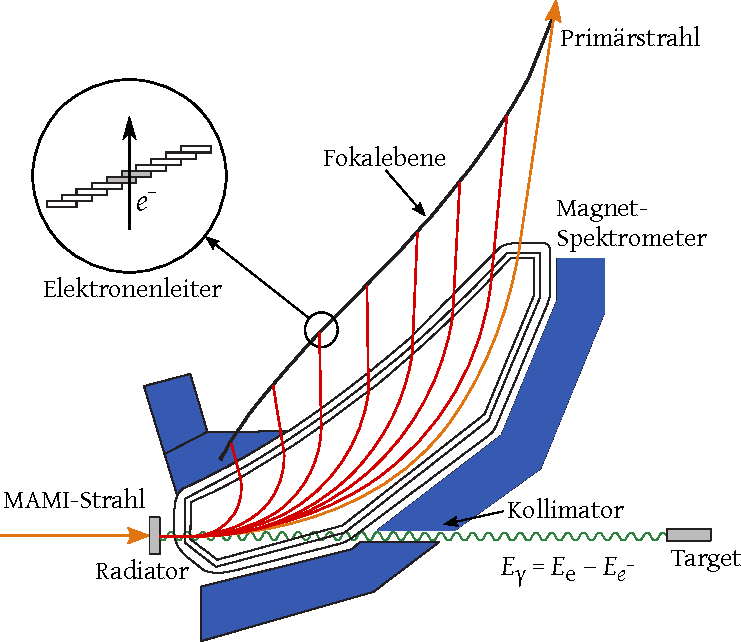
\includegraphics{TAGGER}
	
	\caption{Der Glasgow-Mainz-Tagger: Am Radiator entstanden durch Bremsstrahlung Photonen, welche den Kollimator passierten und auf das Target trafen. Die Elektronen wurden durch den Dipol auf den Elektronenleiter angelenkt, wodurch sich ihre Energie bestimmen lie{\ss}\cite{Un08}}
\label{fig.TAGGER}	
\end{center}
\end{figure}
 
 
\section{Das Detektorsystem}
Nach seiner Erzeugung traf der Photonenstrahl auf das Flüssig-Wasserstoff-Target, welches sich im Zentrum des Crystal-Balls (CB) befand. Die erzeugten und gestreuten Teilchen konnten dann durch ein System von Detektoren bestehend aus dem Crystal-Ball Detektor, einem Teilchenidentifikationsdetektor (PID\footnote{Particle Ideticication Detector}), zwei Vieldrahtproportionalkammern (MWPC\footnote{Multi-Wire Proportional Chamber}) und einem Photonenspektrometer (TAPS\footnote{Two Arm  Photon Spectrometer}) nachgewiesen werden. Der PID und die MWPC waren im Inneren des CB angebracht. Der TAPS wurde am Ausgang des CB platziert, um einen fast vollständig abgedeckten Raumwinkel zu erreichen.
\begin{figure}[h]
	\begin{center}
		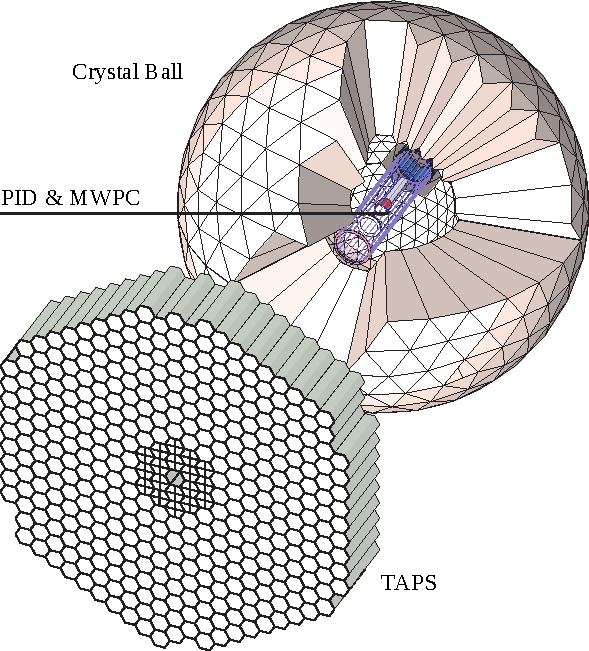
\includegraphics{crystal_ball}
	
		\caption{Anordnung des Detektorsystems: Im Zentrum des sph\"arischen Kalorimeters (CB) befanden sich der Detektor zur Teilchenidentifikation (PID) und zwei zur Bestimmung der Teilchen-Trajektorie (MWPC). Die TAPS-Wand befand sich am Ausgang des CB und sorgte daf\"ur, dass der CB einen Raumwinkel von fast 4$\pi$ abdeckte\cite{We13}}
		\label{[fig.crystal_ball]}	
\end{center}
\end{figure}

\subsection{Der Crystal-Ball-Detektor}
Ursprünglich wurde der Crystal-Ball Detektor Anfang der 70er Jahre am SPEAR\footnote{Stanford Positron Electron Asymmetric Ring} zur Entdeckung des $J/\Psi$-Mesons entwickelt. Später wurde mit seiner Hilfe das Bottom-Quark am DESY\footnote{Deutsches Elektronen-Synchrotron} und Baryonenresonanzen am BNL\footnote{Brookhaven National Laboratory} untersucht.
Seit November 2002 stand der Crystal-Ball Detektor der A2-Kollaboration am MAMI für Experimente mit reellen Photonen zur Verfügung.
\newline
Der Crystal-Ball war ein Kalorimeter bestehend aus 672 Natriumiodid (NaI) Szintillatoren, welche so angeordnet waren, dass 93,3\% des Raumwinkels abgedeckt werden konnte. 
Die Geometrie basierte auf der Form eines Ikosaeders, ein W\"urfel bestehend aus 20 gleichgro{\ss}en  gleichseitigen Dreiecken. Jedes dieser Dreiecke war weiter aufgeteilt in in vier kleinere gleichseitige Dreiecke, welche wiederum jeweils in neun gleichseitige Dreiecke unterteilt waren. Somit ergaben sich 720 gleichseitige Fl\"achen. Aufgrund der hohen Zahl der Fl\"achen erinnerte der Crystal-Ball an eine Hohlkugel mit einem au{\ss}en Radius von ca. 66 cm und einen Innenradius von ca. 25 cm. Da der Crystal-Ball Detektor urspr\"unglich in $e^-e^+$ Streuexperimenten verwendet wurde, mussten sowohl f\"ur den Strahleneingang als auch -ausgang 24 dieser Fl\"achen entfernt werden, wodurch insgesamt 672 Detektoren angebracht werden konnten. Die NaI-Szintillatorkristalle waren ca. 40 cm ($\sim$15,7 Strahlungsl\"angen) lang, hatten die Form eines Pyramidenstumpfes mit dreieckiger Grundfl\"ache und einer Seitenl\"ange von etwa 5 cm am schmalen und ca. 13 cm am dicken Ende. Jeder dieser Kristalle deckte etwa 0,14 \% des Raumwinkels ab und wurde durch einen eigenen Photoelektronenvervielfacher (PTM\footnote{PhotoMultiplier-Tube}) ausgelesen. 



\subsection{TAPS, PID \& MWPC}
Der PID hatte eine zylindrische Form mit einem Durchmesser von 116,5 mm und bestand aus 24 einzelnen Szintillatoren, welche jeweils 500 mm lang, 15,3 mm breit und 4 mm dick waren. Da die Szintillatoren nur eine geringe Dicke aufwiesen, verloren Photonen beim durchfliegen weniger als 1\% ihrer Energie. Geladene Teilchen auf der anderen Seite erfuhren einen Energieverlust $\Delta E$. Ihre restliche Energie wurde im Crystal-Ball abgegeben. Folglich konnte der PID zwischen geladenen und ungeladenen Teilchen unterscheiden. 
Au{\ss}erhalb des PIDs waren die MWPCs angebracht. Dabei handelte es sich um zwei, aus Anodendr\"ahten aufgebauten, Ioniastionskammern in Form von Zylindern. Die Anodendr\"ahte waren parallel zur Strahlenachse ausgerichtet und befanden sich zwischen zwei Lagen von spiralf\"ormigen Kathodenstreifen. 
Da die A2-Kollaboraions Experimente mit einem Fixed-Target untersucht und der Crystal-Ball zwei \textit{L\"ocher} f\"ur einen Strahleneingang und -ausgang besa{\ss}, wurde die TAPS-Wand entwickelt. Diese deckte einen Vorw\"artswinkel zur Strahlenachse von 1,2 ° bis 20 ° ab. Sie wurde etwa 1,5 m vom Mittelpunkt des CB entfernt positioniert und bestand aus 72 PbWO$_4$ und 366 BaF$_2$ Szintillatorkristallen. Somit konnte mit diesem Detektorsystem ein Raumwinkel von fast 97\% abgedeckt werden.


\chapter{Studien zur Kalibrierung des Crystal-Ball}

\section{Energie-Interval Abhängigkeit}

Zunächst wurde überprüft, ob es eine Abhängigkeit der Kalibrierung im Bereich verschiedener Energieintervalle gab. Sprich, stimmt die Kalibrierung auch dann noch, wenn die Energie der beiden detektierten Photonen sich ähnelte. Dazu wurden die Daten der Strahlzeit aus dem Jahr 2014 genommen. Aus diesen Daten konnte mit der Gleichung
\begin{equation}
m_{\pi^0}=\sqrt{2E_{\gamma_1}E_{\gamma_2}(1-cos(\theta))}
\label{eq:invariantmass}
\end{equation}
die invariante Masse des $\pi^0$ berechnet werden. Dabei sind $E_{\gamma_1}$ und $E_{\gamma_2}$ die Energien der beiden Photonen und $\theta$ ist der Winkel, zwischen den beiden Photonen. 
Damit konnte dann ein zweidimensionales Histogramm angelegt werden, mit der invarianten Masse auf der x-Achse. Auf der y-Achse wurde die Energie der Photonen aufgetragen, welche in Intervalle mit einer Breite von 25 MeV unterteilt wurden. 


\begin{figure}[h]
	\begin{center}
		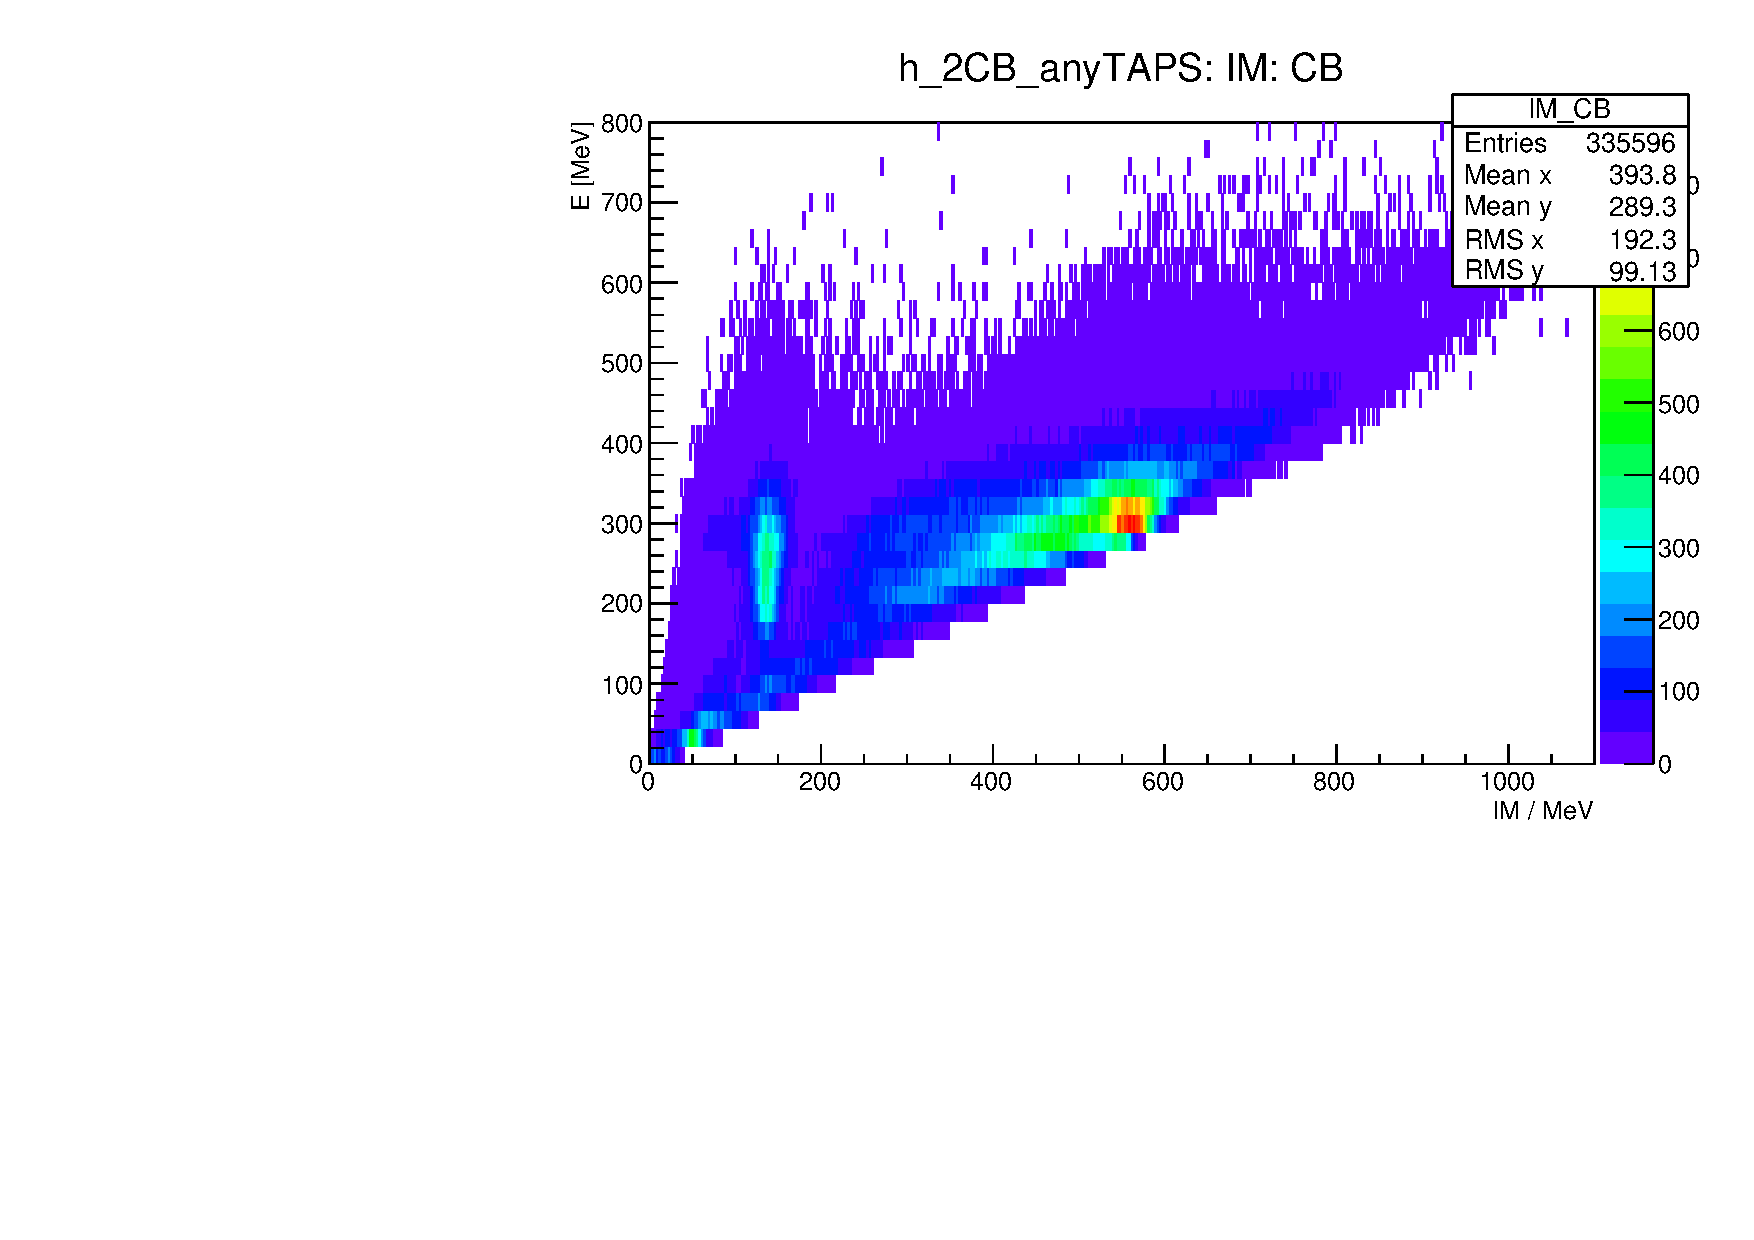
\includegraphics[width=100mm]{energydependencyallbins0903}
	
		\caption{2-D Histogram: Auf der x-Achse ist die errechnete invariante Masse aufgetragen, die y-Achse ist in 25 MeV Intervalle aufgeteilt. Es wurden nur dann die Invariante Masse errechnet, wenn sich die Energie beider Photonen im gleichen Interval befanden.}
			\label{fig:Energy-Interval-Hist-All-Bins}
	\end{center}
\end{figure}

Beim Füllen des Histogramms wurde darauf geachtet, dass sich die Energien der beiden Photonen im gleichen Intervall befanden.

Formel \ref{eq:invariantmass} gibt auch die untere Energiegrenze zur Entstehung von $\pi^0$ an. Aufgrund der Geometrie des Crystal-Balls konnten nicht alle Winkel abgedeckt werden. So deckten die Detektoren nur einen Winkelbereich von etwa 20°-160° zur Strahlenachse ab. Wählt man nun für $m_{\pi^0}$ den Literaturwert 135 MeV und setzt $E_{\gamma}=E_{\gamma_1}=E_{\gamma_2}$ und $\theta= 20$°, dann kann man nach $E_{\gamma}$ auflösen und erhält $E_{\gamma}$ = 114 MeV. Das heißt, erst wenn beide Photonen eine Energie von mindestens 114 MeV besitzen, können $\pi^0$-Mesonen erzeugt werden. Allerdings mussten auch die Intervalle von 100 bis 150 MeV verworfen werden, da hier der $\pi^0$-Peak zu stark durch den Untergrund gest\"ort wurde. Für Energien über 450 MeV gab es nicht mehr genug Ereignisse, wodurch diese Energieintervalle auch verworfen werden mussten. Deswegen wurden in den folgenden Betrachtungen nur Energieintervalle im Bereich von 150 MeV bis 450 MeV berücksichtigt.
Um nun die Position des $\pi^0$ zu bestimmen, wurde für jedes Intervall über den Bereich von 70 MeV bis 180 MeV gefittet. 


\begin{figure}[h]
	\begin{center}
		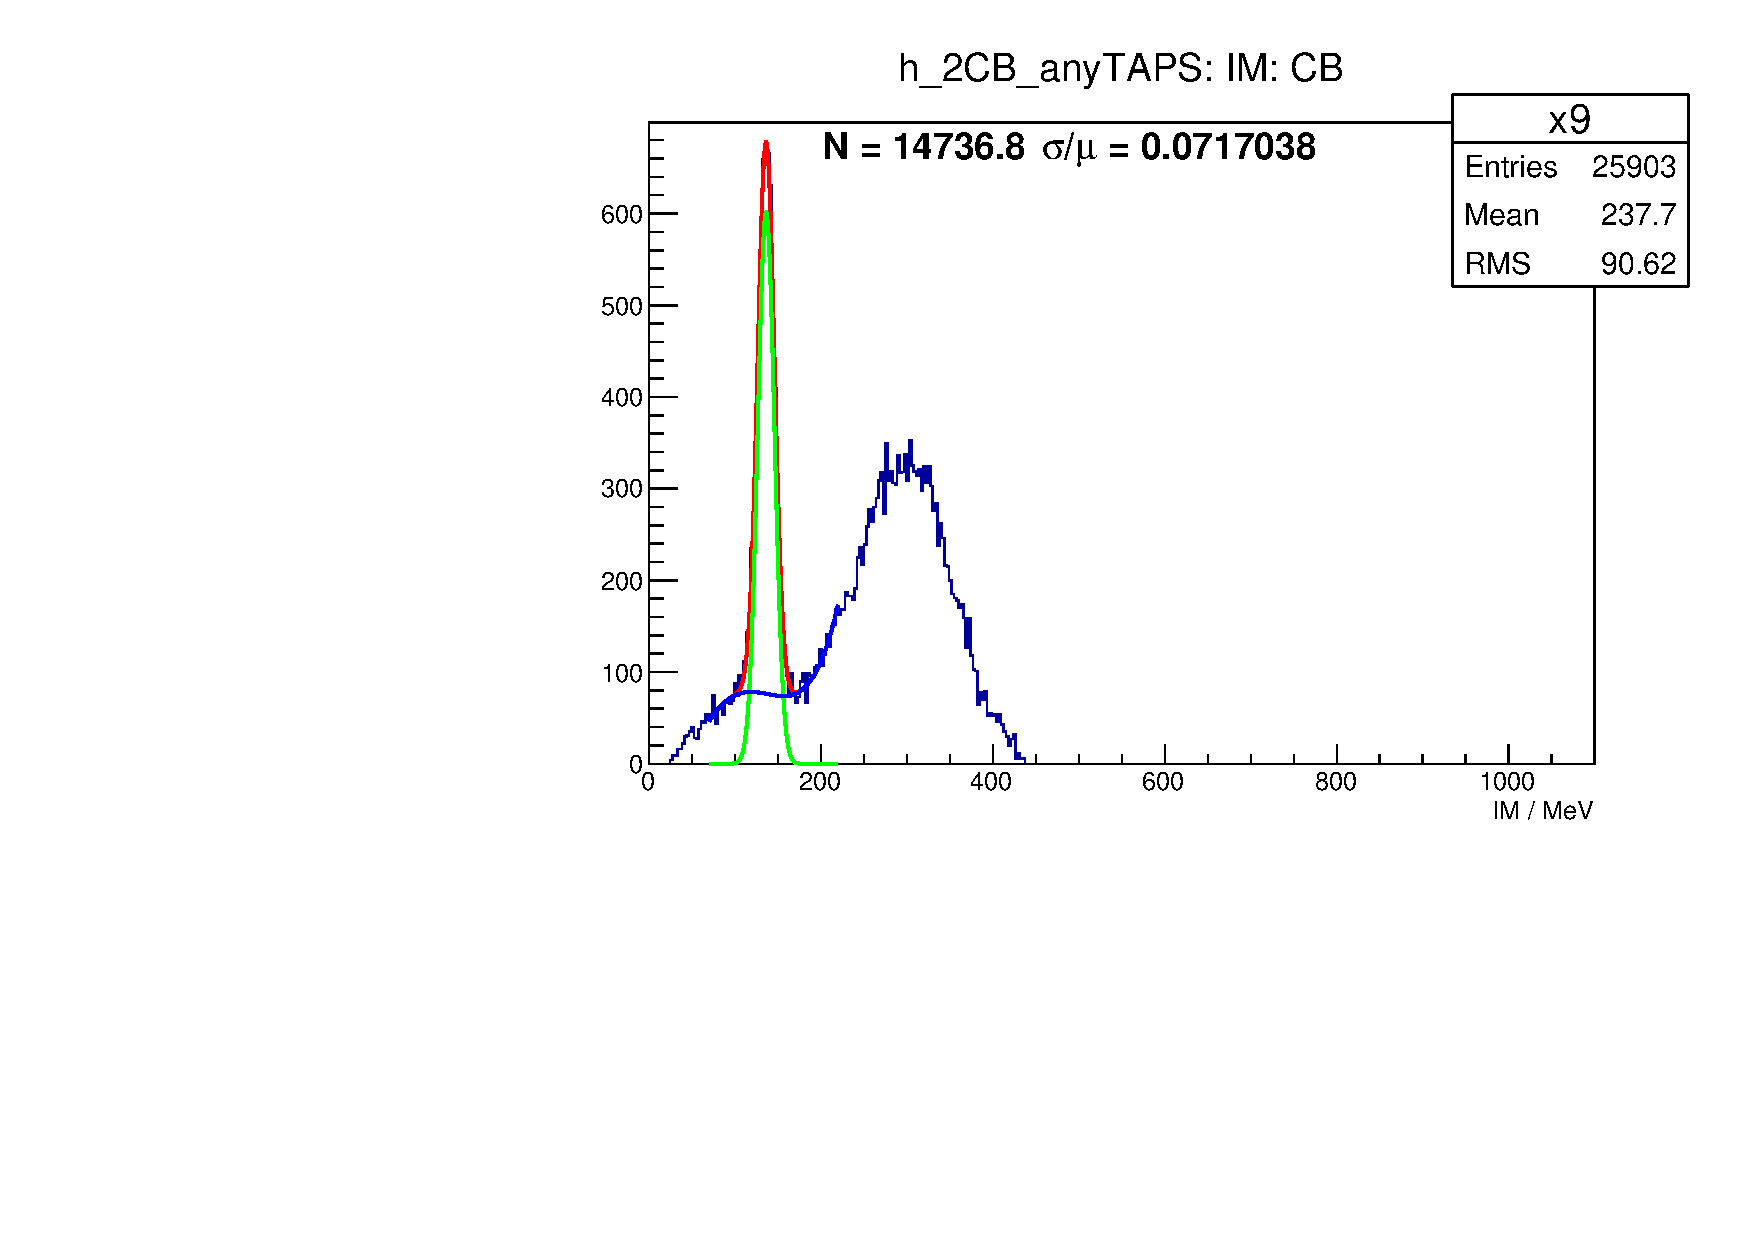
\includegraphics[width=100mm]{fitexampleenergyinterval0903}
		
		\caption{Beispiel eines Fits. Es handelt sich dabei um das Energieintervall von 200 MeV bis 225 MeV}
		\label{fig:fitexampleenergyinterval0903}	
\end{center}
\end{figure}
 Beim Fit wurde zuerst der Untergrund mit einem Polynom vierten Grades gefittet, in Abbildung \ref{fig:fitexampleenergyinterval0903} blau dargestellt. Von den Daten konnte damit der Untergrund abgezogen werden, was den einen besseren Gauß-Fit (grün) des Peaks ermöglichte. Daraus konnte die Position des $\pi^0$-Peaks abgelesen werden. 
 
 \begin{figure}[h]
 	\begin{center}
 		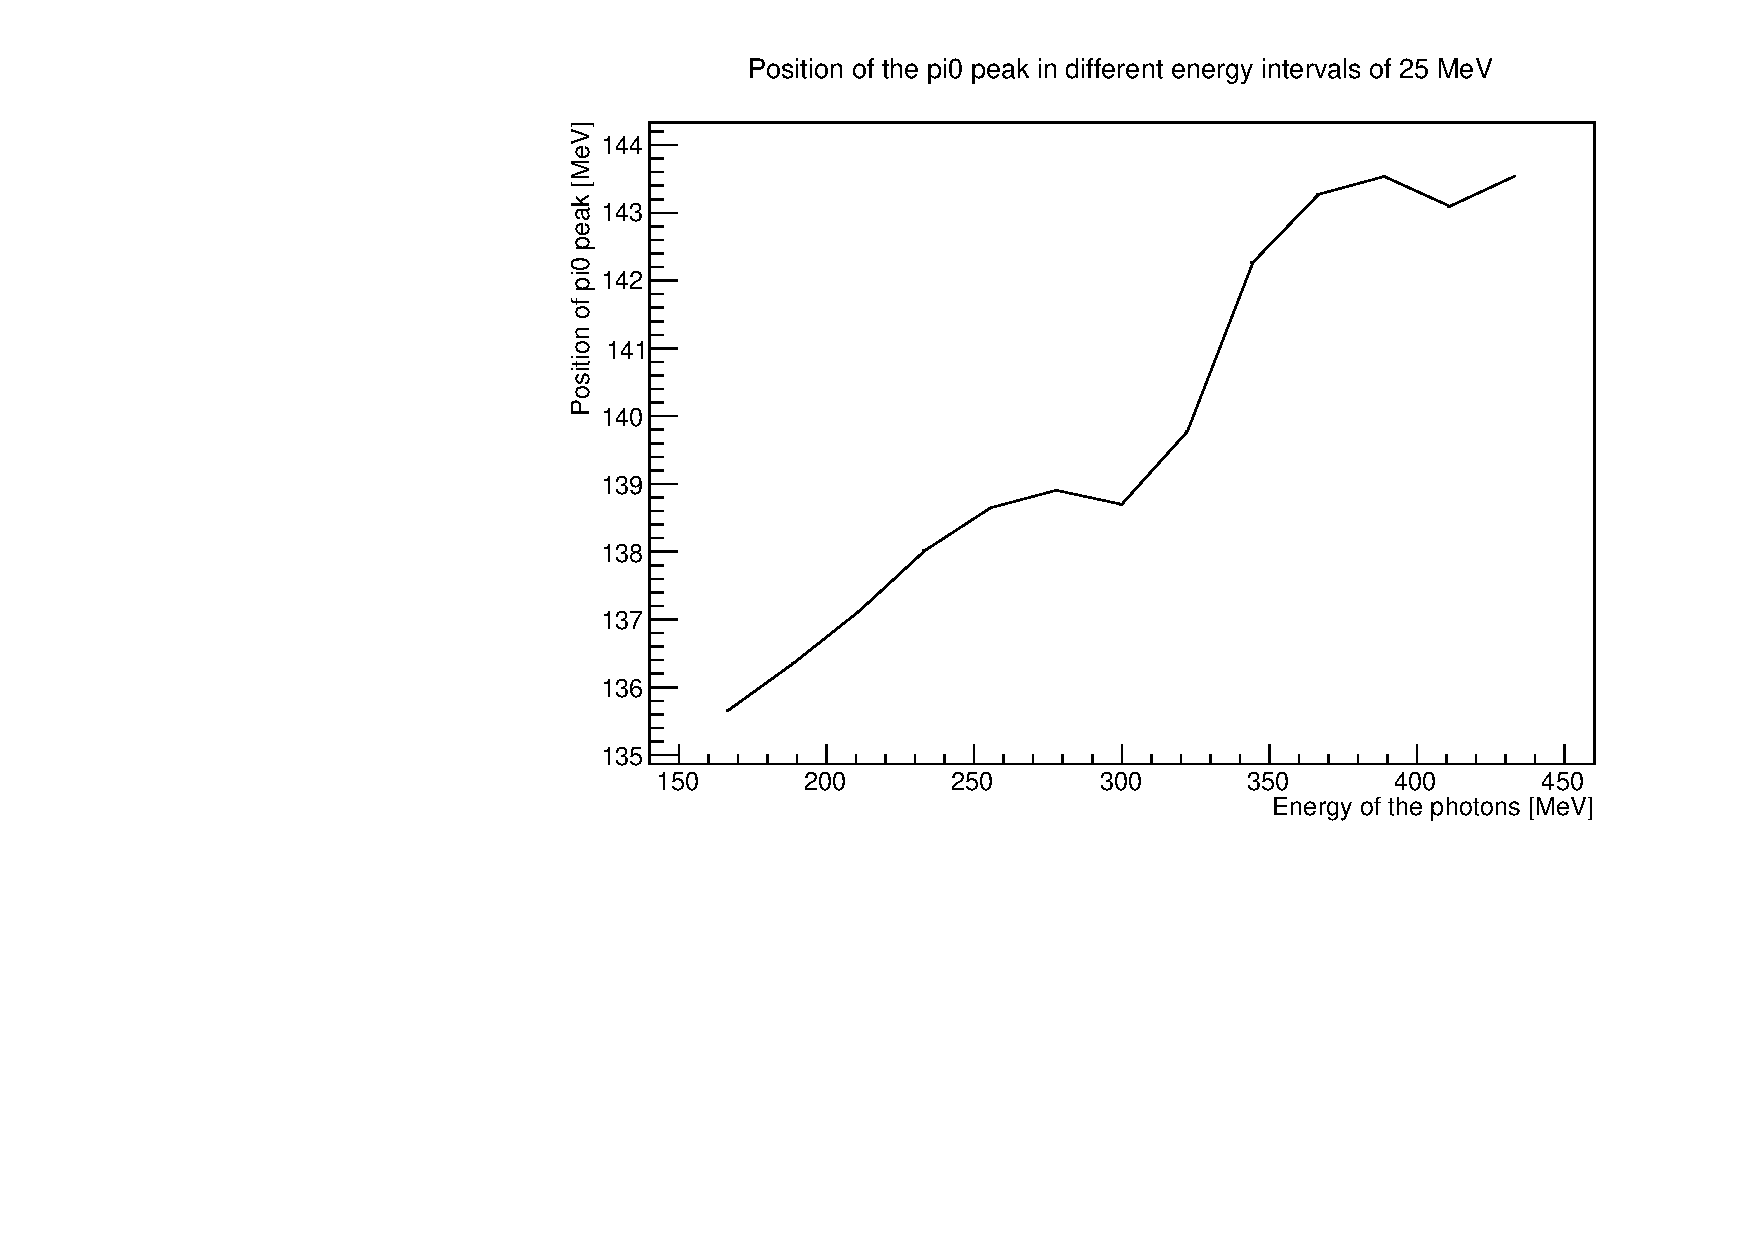
\includegraphics[width=100mm]{energydependency0903}
 	
 		\caption{Position der $\pi^0$ aus Abbildung \ref{fig:Energy-Interval-Hist-All-Bins}. Die errechnete Position des $\pi^0$ Peaks wurde gegen die Energie der Photonen aufgetragen. Gr\"o{\ss}ere Energieintervalle wurden aufgrund zu kleiner Statistik nicht ber\"ucksichtigt. F\"ur kleinere Energien konnten keine $\pi^0$ Teilchen erzeugt werden} 
 		\label{fig.Energydependency_pion}
 	\end{center}
 \end{figure}
  
In Abbildung \ref{fig.Energydependency_pion} wurden die errechneten Positionen der Pionen gegen die Energie der Photonen aufgetragen. Zu sehen ist eine deutliche Abweichung zum Literaturwert des $\pi^0$ Peaks. Auch nahm die Abweichung für größere Energien zu und betrug teilweise über 6\% (vgl. Abb.:\ref{fig:RelativEnergyDependency}).
  
Daraus folgte, dass eine Abhängigkeit zwischen der Position des $\pi^0$-Peaks und der Energie vorlag, wenn sich die Photonen energetisch ähnelten.



%_______________________________________________________________________________
\chapter{Zusammenfassung und Ausblick}

In der Zusammenfassung sollten Sie in knapper Form die Aufgabenstellung 
und die wichtigsten Ergebnisse rekapitulieren. Es ist f\"ur die 
Gutachter hilfreich, wenn Sie ausdr\"ucklich beschreiben, worin 
Ihre eigenen Beitr\"age liegen. Scheuen Sie sich auch nicht davor 
auszusprechen, welche Untersuchungen durch die Zeitbegrenzung der 
Bachelorarbeit nicht m\"oglich waren und nutzen Sie dies als 
\"Uberleitung zu einem Ausblick auf m\"ogliche weitergehende 
Arbeiten an der Aufgabenstellung.

%_______________________________________________________________________________
\begin{appendix}
\chapter{Anhang Nummer 1}

\section{Tabellen und Abbildungen}

In der Regel sind die in Tabellen und Abbildungen enthalten Informationen 
so wichtig, dass sie im Hauptteil der Arbeit erscheinen sollten. Unter 
Umst\"anden sind aber erg\"anzende Tabellen und Abbildungen gut in einem 
Anhang aufgehoben. Wie im Hauptteil sollten Sie auch hier darauf achten, 
dass die in Tabellen und Figuren (siehe Abb.\ \ref{Abb:1}) dargestellte 
Information im Text angesprochen wird und selbsterkl\"arende Legenden 
vorhanden sind.
\medskip






\begin{figure}[h]
	\begin{center}
		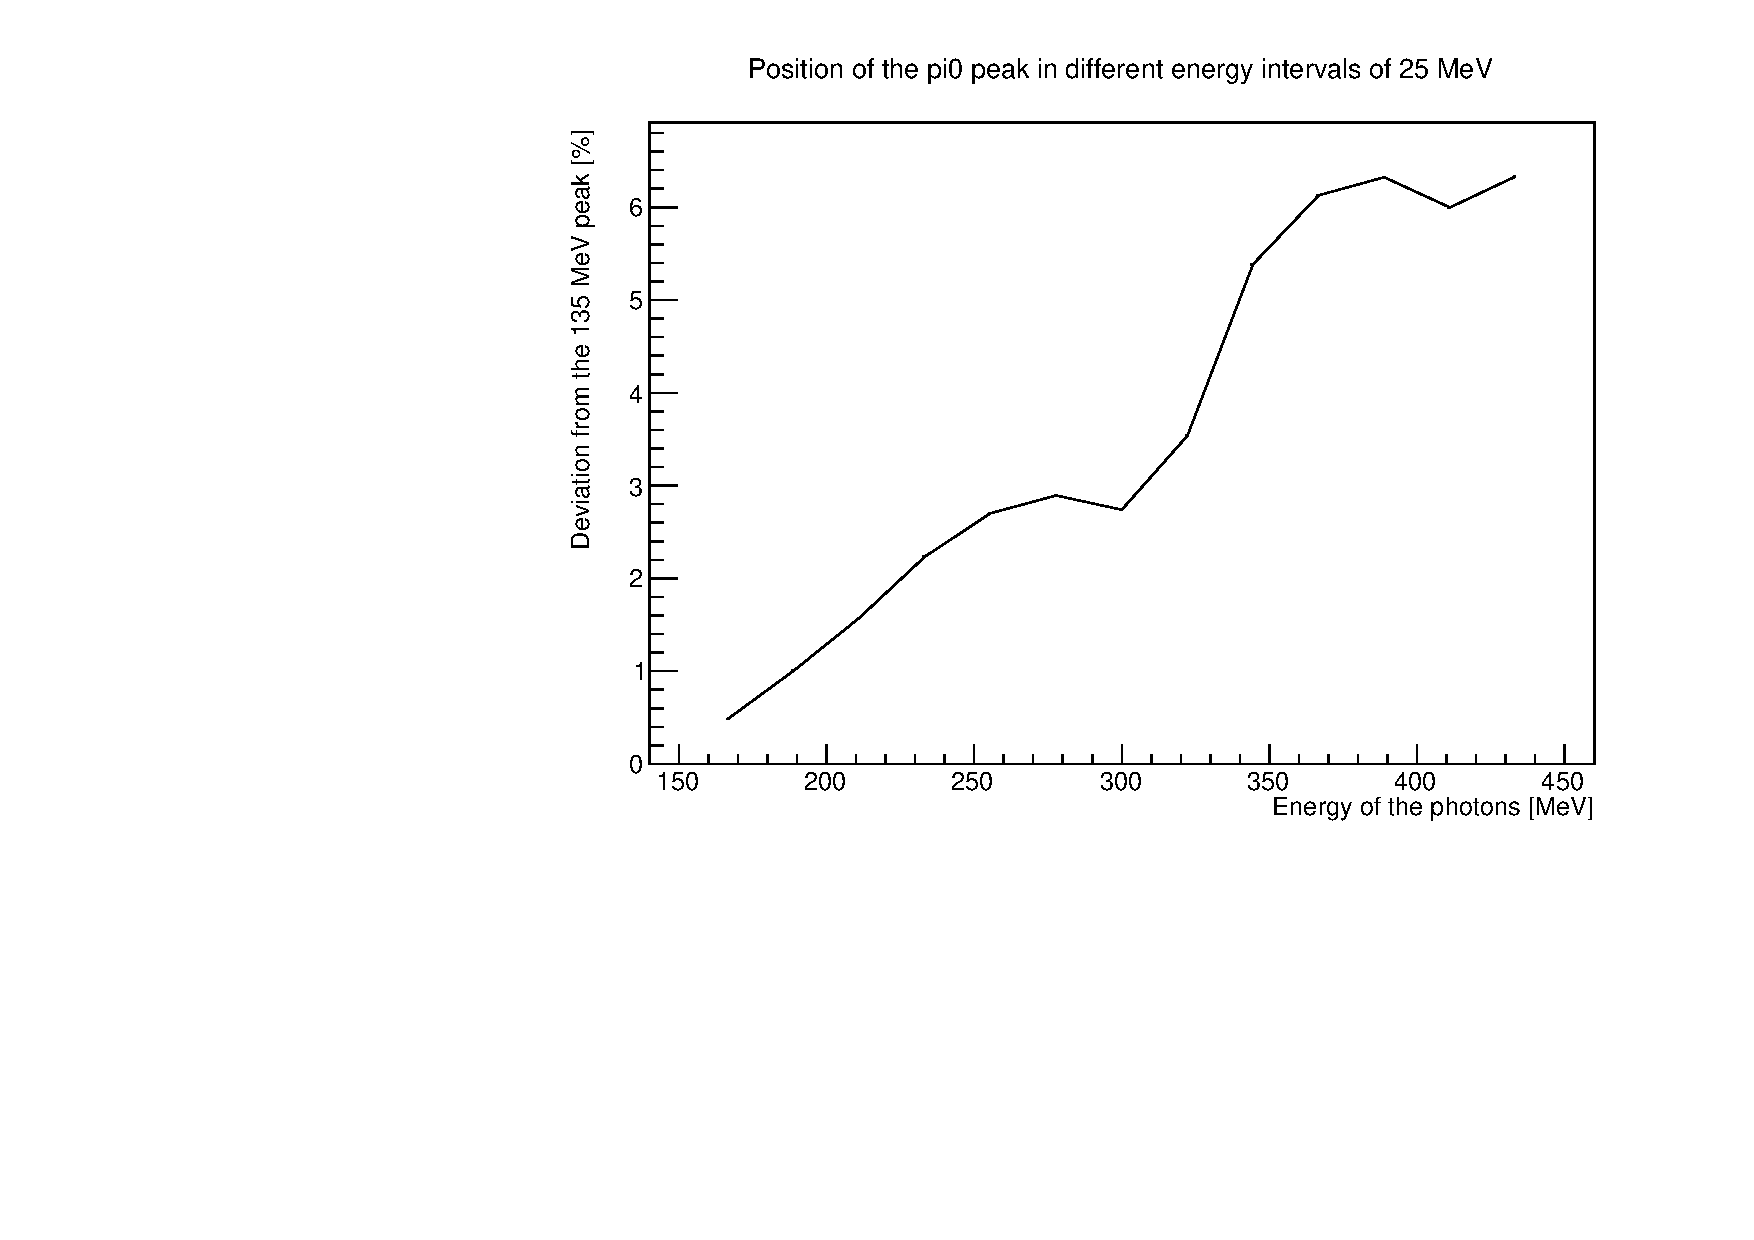
\includegraphics[width=100mm]{relativedependency0903}
		
		\caption{Die relative Abweichung des errechneten $\pi^0$-Peaks aus Abbildung \ref{fig:Energy-Interval-Hist-All-Bins} von dem Literaturwert. Die Abweichung wurde in Prozent gegen die Energie der Photonen aufgetragen.  Position des $\pi^0$ Peaks wurde gegen die Energie der Photonen aufgetragen. Gr\"o{\ss}ere Energieintervalle wurden aufgrund zu kleiner Statistik nicht ber\"ucksichtigt. F\"ur kleinere Energien konnten keine $\pi^0$ Teilchen erzeugt werden}			
		\label{fig:RelativEnergyDependency}	
	\end{center}
\end{figure}

%_______________________________________________________________________________
\section{Weiterf\"uhrende Details zur Arbeit}

Manch wichtiger Teil Ihrer tats\"achlichen Arbeit ist zu technisch 
und w\"urde den Hauptteil des Textes un\"ubersichtlich machen, 
beispielsweise wenn es um die Details des Versuchsaufbaus in einer 
experimentellen Arbeit oder um den f\"ur eine numerische Auswertung 
verwendeten Algorithmus geht. Dennoch ist es sinnvoll, entsprechende 
Beschreibungen in einem Anhang Ihrer Bachelorarbeit aufzunehmen. 
Insbesondere f\"ur zuk\"unftige Arbeiten, die an Ihre Bachelorarbeit 
anschlie{\ss}en, sind dies manchmal hilfreiche Informationen.

%_______________________________________________________________________________
\chapter{Literaturverzeichnis}

Machen Sie genaue Angaben, so dass die verwendeten Literaturstellen 
eindeutig identifiziert und aufgefunden werden k\"onnen.
Bei Lehrb\"uchern \cite{Weinberg:1995mt} ist es sinnvoll, 
den Titel anzugeben, eventuell auch die Ausgabe. Bei Artikeln in 
Fachzeitschriften \cite{Moch:2001zr} ist es \"ublich, nur die 
gebr\"auchlichen Abk\"urzungen f\"ur den Titel der Zeitschrift, Band, 
Erscheinungsjahr und Seite anzugeben. Unter Umst\"anden kann es auch 
sinnvoll sein, im Internet aufgefundene Informationsquellen anzugeben, 
zum Beispiel f\"ur Software \cite{LoopTools} oder zu den Details von 
Ergebnissen gro{\ss}er experimenteller Kollaborationen. Es ist 
selbstverst\"andlich, dass Sie auch Bachelor- \cite{BA:Freund}, 
Diplom- oder Doktorarbeiten angeben, wenn Sie diese in Ihrer eigenen 
Arbeit verwendet haben.
\medskip



\renewcommand{\bibname}{\bfont Literaturverzeichnis} 
\bibliographystyle{h-physrev3}
\begin{thebibliography}{99}
	
\bibitem[Un04]{Un04} Diplomarbeit von Marc Unverzagt, 2004 {\em Energie-Eichung des Crystal-Ball-Detektors am MAMI}
\bibitem[Un08]{Un08} Dissertation von Marc Unverzagt, 2008 {\em Bestimmung des Damitz-Plot-Parameters $\alpha$ für den Zerfall $ \eta 3\pi^{0} $ mit dem Crystal Ball am MAMI}
\bibitem[We13]{We13} Diplomarbeit von Jennifer Wettig, 2013 {\em Aufbau und Inbetriebnahme einer neuen HV-Versorgung für den Crystal Ball Detektor am MAMI}
\bibitem[KPh11G]{KPh11G} Internetseite der Kernphysik {\em Mainzer Mikrotron-Geschichte}, Internetseite \url{http://www.kernphysik.uni-mainz.de/379.php}, (Stand 04.03.2017)
\bibitem[KPh11F]{KPh11F} Internetseite der Kernphysik {\em Funktionsprinzip des MAMI}, Internetseite \url{http://www.kernphysik.uni-mainz.de/375.php}, (Stand 06.03.2017)

\bibitem[KPh04]{KPh04} Prospekt des Institut für Kernphysik Internetlink, \url{https://portal.kph.uni-mainz.de/de/information/introduction/prospekt.pdf}, (Stand: 04.03.2017)

\bibitem[KPh07]{KPh07} Pressemitteilung der KPh, \url{https://www.uni-mainz.de/presse/archiv/zope.verwaltung.uni-mainz.de/presse/mitteilung/2007/2007_10_05_phys_einweihung_mami/showArticle_dtml.html}, (Stand 06.03.2017)
\bibitem[KPh16]{KPh16} Internetseite der A2-Kollaboration {\em Reelle Photonen}
Internetseite {\url http://www.kph.uni-mainz.de/a2.php} (Stand 11.03.2017)











%\cite{BA:Freund}
\bibitem{BA:Freund}
  B.~Freund Nummer eins, 
  Bachelorarbeit, Johannes Gutenberg-Universit\"at Mainz, 2012.

\end{thebibliography}

%_______________________________________________________________________________
\chapter{Danksagung}

... an wen auch immer. Denken Sie an Ihre Freundinnen und Freunde, 
Familie, Lehrer, Berater und Kollegen.

\end{appendix}


\end{document}  
        
        